\documentclass[crop,tikz]{standalone}
\usetikzlibrary{backgrounds}
\colorlet{blue}{cyan}
\tikzset{
  inverted/.style = {
    color=white,
    background rectangle/.style={fill},
    show background rectangle
  }
}

\tikzset{>=latex}
\usetikzlibrary{decorations.markings}
\colorlet{green}{green}
\definecolor{orange}{RGB}{250,194,25}
\newcommand{\place}{\vec{r}}
\newcommand{\acceleration}{\vec{a}}

\begin{document}
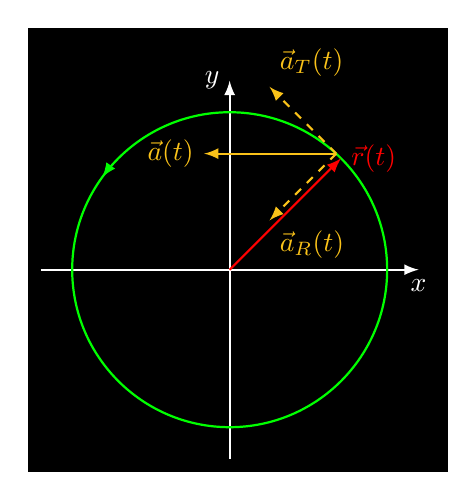
\begin{tikzpicture}[inverted,scale=2]
  \draw[->,thick] (-1.2,0) -- (1.2,0) node[below] {$x$};
  \draw[->,thick] (0,-1.2) -- (0,1.2) node[left] {$y$};
  \draw[
    decoration={markings, mark=at position 0.4 with {\arrow{>}}},
    postaction={decorate},
    green,
    thick
  ] (0,0) circle (1);
  \draw[->,thick,red] (0,0) -- (45:1) node[right]{$\place(t)$};
  \begin{scope}[shift={(-0.03,0.03)}]
    \draw[->,thick,orange,dashed] (45:1) -- +(135:0.6) node[left,anchor=south west]{$\acceleration_T(t)$};
    \draw[->,thick,orange,dashed] (45:1) -- +(225:0.6) node[right,anchor=north west]{$\acceleration_R(t)$};
    \draw[->,thick,orange] (45:1) -- +(180:0.84) node[left]{$\acceleration(t)$};
  \end{scope}
\end{tikzpicture}
\end{document}
